\documentclass[12pt,a4paper]{article}
\usepackage[latin1]{inputenc}
\usepackage{amsmath,bm}
\usepackage{amsfonts}
\usepackage{amssymb}
\usepackage{makeidx}
\usepackage{graphicx}
\usepackage{float}
\usepackage{color}
\usepackage{xcolor}
\usepackage[colorlinks,linkcolor=blue,anchorcolor=blue,citecolor=blue]{hyperref}
\usepackage{amsmath,amsthm,amssymb}

\usepackage[level]{datetime}

%\usepackage{wasysym}
%\usepackage{marvosym}

%\usepackage{ctexcap}

\usepackage{amsmath}
\usepackage{amssymb}
\usepackage{array}
\usepackage{amsmath,subfigure}%,psfig
\usepackage{algorithm}
\usepackage{booktabs}
\usepackage{multirow}
\usepackage{colortbl}
\definecolor{tabcolor}{rgb}{.105,.410,.113}


\usepackage{geometry}
\geometry{left=2.5cm,right=2.5cm,top=2.5cm,bottom=2.5cm}
\linespread{1.25}
%\linespread{1.05}
\setlength{\parskip}{0.5\baselineskip}

\usepackage{lastpage}%获得总页数

%\addtolength{\hoffset}{-1.2cm}%增加左边距-2cm
%\addtolength{\voffset}{-1.5cm}%增加上边距-3cm
%\addtolength{\textwidth}{2.4cm}%增加文本区域宽度4cm
%\addtolength{\textheight}{3cm}%增加文本区域高度5cm


\usepackage[center]{titlesec}
\renewcommand{\thefootnote}{\fnsymbol{footnote}}
\renewcommand{\baselinestretch}{1.1}%{1.2}
\newcommand{\dachu}{\fontsize{48pt}{\baselineskip}\selectfont}
\newcommand{\chuhao}{\fontsize{42pt}{\baselineskip}\selectfont}
\newcommand{\xiaochuhao}{\fontsize{36pt}{\baselineskip}\selectfont}
\newcommand{\yihao}{\fontsize{28pt}{\baselineskip}\selectfont}
\newcommand{\xiaoyihao}{\fontsize{24pt}{\baselineskip}\selectfont}
\newcommand{\erhao}{\fontsize{21pt}{\baselineskip}\selectfont}
\newcommand{\xiaoerhao}{\fontsize{18pt}{\baselineskip}\selectfont}
\newcommand{\sanhao}{\fontsize{15.75pt}{\baselineskip}\selectfont}
\newcommand{\xiaosanhao}{\fontsize{15pt}{\baselineskip}\selectfont}
\newcommand{\sihao}{\fontsize{14pt}{\baselineskip}\selectfont}
\newcommand{\xiaosihaomore}{\fontsize{13pt}{1.12\baselineskip}\selectfont}
\newcommand{\xiaosihao}{\fontsize{12pt}{1.12\baselineskip}\selectfont}
\newcommand{\xiaosihaoless}{\fontsize{12pt}{0.8\baselineskip}\selectfont}
\newcommand{\wuhao}{\fontsize{10.5pt}{\baselineskip}\selectfont}
\newcommand{\xiaowuhao}{\fontsize{9pt}{\baselineskip}\selectfont}
\newcommand{\liuhao}{\fontsize{7.875pt}{\baselineskip}\selectfont}
\newcommand{\qihao}{\fontsize{5.25pt}{\baselineskip}\selectfont}

\renewcommand{\normalsize}{\xiaosihao}%less}

\titleformat{\section}{\sihao\bfseries}{\thesection}{1em}{}
\titleformat{\subsection}{\xiaosihaomore\bfseries}{\thesubsection}{1em}{}
\titleformat{\subsubsection}{\xiaosihaomore\bfseries}{\thesubsubsection}{1em}{}

\title{User Manual of TeXpen}
\author{MengChang Wang}

\newcommand{\upcite}[1]{\textsuperscript{\cite{#1}}}

\newcommand{\texpen}{{\TeX}pen~}

%\newdateformat{ukdate}{\ordinaldate{\THEDAY} \monthname[\THEMONTH] \THEYEAR}%日月年

%\renewcommand{\today}{\number\day, \number\month, \number\year}

\renewcommand{\today}{\number\day,\space\ifcase\month\or
Jan\or Feb\or Mar\or Apr\or May\or Jun\or
Jul\or Aug\or Sep\or Oct\or Nov\or Dec\fi,
\space\number\year}

\usepackage{fancyhdr}
\pagestyle{fancy}
\fancyhf{}
\fancyhead[L]{\color{gray}{ \textit{User Manual of {\TeX}pen }}}%
\includegraphics[width=3.0cm]{figs/texpen.png}}
\fancyhead[R]{
\includegraphics[width=0.8cm]{figs/texpen.png}}%{\empty}%\textit{Survey Report\\$\;$}}
\fancyfoot[R]{\thepage/\pageref{LastPage}}%{Page \thepage/8}
\fancyfoot[L]{\scriptsize\textit{		
		\today %插入当前日期
	}}%School of Mechanical \& Aerospace Engineering}}
\renewcommand{\headrulewidth}{1pt} 
\setlength{\headsep}{0.8cm}


%%%%%%%%%TikZ
\usepackage{pgf}
\usepackage{tikz}
\usetikzlibrary{arrows,automata}
\usetikzlibrary{positioning}
%%%%%%%%%TikZ

%\usepackage{fontspec}
%\usepackage{charter}
\usepackage{mathpazo}
%\setmainfont{Liberation Serif}%[BoldFont=SimHei]{Palatino}



\renewcommand{\contentsname}{CONTENTS}
\renewcommand{\refname}{REFERENCES}



%%%%%%%%%%%%%%%%%%%%%%%%%%%%%%%%%%%%%%%%%%%%%
%%%%%%%%%%%%%%%%%%%%%%%%%%%%%%%%%%%%%%%%%%%%%
%%%%%%%%%%%%%%%%%%%%%%%%%%%%%%%%%%%%%%%%%%%%%

\begin{document}

%\maketitle


%%%%%%%%%%%
%% Cover Page %%

%\pagestyle{plain}
\thispagestyle{empty}
$\;$\\

\begin{flushright}
\begin{tabular}{l}
\arrayrulecolor{tabcolor}
\toprule [1pt]
\\
\xiaoerhao {User Manual of {\TeX}pen }\\ [1.2ex]
\\
\hline
$\;$\\ [1.2ex]
\sihao {Dr. WANG MengChang and Dr. SHAN Dan} \\ [1.2ex]
\\
\hline
$\;$\\ [1.2ex]
\wuhao {wangmengchang@gmail.com } \\ [1.2ex]
\\
\bottomrule [1pt]
\end{tabular}
\end{flushright}

\vfill


\begin{picture}(1,1)
\put(-20,-3){
\includegraphics[width=3cm]{figs/texpen.png}}
\end{picture}

%\begin{picture}(1,1)
%\put(300,-2.5){\includegraphics[width=4.8cm]{figs/ntu.png}}
%\end{picture}

%\noindent
%\begin{flushright}
% \includegraphics[height=1.8cm]{figs/ntu.png}\\
%\end{flushright}

\clearpage
\setcounter{page}{1}
\thispagestyle{empty}

$\;$


\vspace{6cm}

%I have a dream, where the computer helps me thinking, but I twinkle the cursor. 
I have a dream, where the computer helps me think, but I twinkle the sparks in my eyes. 

\begin{picture}(1,1)
\put(90,-90){
\includegraphics[width=6cm]{figs/eye.png}}
\end{picture}



\clearpage
\setcounter{page}{1}
\pagestyle{fancy}


\tableofcontents
\clearpage
%\listoftables       %表目录
%\clearpage
\listoffigures     %图目录



\clearpage
\setcounter{page}{1}


\section{Introduction}

{\TeX}pen is an editor started when Dr. Wang was preparing for his manuscript in his days as a PhD student. Later on, it was improved so that his PhD dissertation can be written with it, including 100,000 Chinese characters with all kinds of equations, figures and tables.

{\TeX}pen aims at lessening the burden of scientific writers in preparing articles, slides and books, and it is still in perhaps endless development and improvement. However, just like any of the majority of those open source projects, {\TeX}pen is provided free of charge, free of guarantee, free of promise, and free of restriction, but full of tiny bugs, full of thirsty for donations, and full of desires for feedbacks.

{\TeX}pen is an editor, or hopefully, an integrated development environment (IDE) for writing Latex based articles and slides. It allows users to finish all works of writing with this single tool, and calls \TeX /\LaTeX functionalities automatically whenever necessary.


\section{Environment \& Installation}

{\TeX}pen is an editor, and users can use it to edit any text file, including plain text files, c plus plus source files, and HTML source files among others. However, it would be happier if users use it for \LaTeX editing. So, it's better to have a \TeX /\LaTeX ~environment, although \texpen is able to work functionally without it.

Users can either compile the source code to get the executable, or directly use the executable for your operating system (OS). We will go through the compilation procedure, but please feel free to skip them if an executable is available. We use Windows OS as an example for illustration, while operations in other OS will be added later.


\subsection{Compilation}
Since {\TeX}pen is developed under Qt, the compilation of {\TeX}pen requires Microsoft Visual Studio (VS) and Qt. VS provides the C/C++ compilier for Qt, while Qt generates the execuble. Users may skip this sub-section if an execuble is alreay available.

\subsubsection{Installation of Visual Studio}
VS 2017 (Community Edition) or later version will be installed first. To save disk space, users may install only C++ related components, including VC++ and Windows SDK, as shown in figure \ref{vs1}.

\begin{figure}[hbt]
\begin{center}
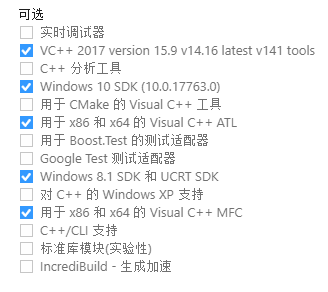
\includegraphics[scale=0.8]{figs/vs1.png}
\end{center}
\caption{The required components of Visual Studio}
\label{vs1}
\end{figure}

\subsubsection{Installation of Qt}
\label{sec:qt}
Qt 5.5 or later version is recommended. While installing Qt, it's important to select the right compilier, or the source codes of {\TeX}pen fail to compile. Qt has built-in compiliers like MinGW, but we need MSVC to compile the component  WebEngine that is used by {\TeX}pen. As a result, both MSVC and WebEngine should be checked while selecting compunents during installation, as shown in figures \ref{qt1} and \ref{qt2}.

\begin{figure}[hbt]
\begin{center}
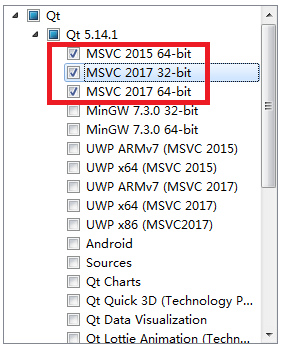
\includegraphics[scale=0.8]{figs/qt1.png}
\end{center}
\caption{The required compiler for Qt}
\label{qt1}
\end{figure}

\begin{figure}[hbt]
\begin{center}
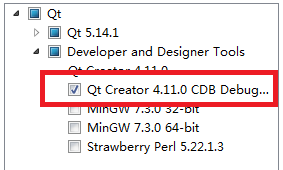
\includegraphics[scale=0.8]{figs/qt2.png}
\end{center}
\caption{The required components of Qt}
\label{qt2}
\end{figure}

\subsubsection{Compilation}
Now it's time to compile the source codes of {\TeX}pen. Locate the file 'texpen.pro' in 'src' folder, open it with Qt Creator, and simply build the project. The executable of {\TeX}pen will be generated if there is no error. If errors happen, please check the installation procedures carefully as introduced in the sub-section.

\subsection{The Latex Environment}
To write a Latex based article or slide using {\TeX}pen, the Latex software Texlive 2018 or later version is recommended for installation. After that, {\TeX}pen is ready to use. 

To check the completion of installation, locate the source code 'docs/manual.tex' of this manual, open it with {\TeX}pen, and try to compile it. If a pdf file exactly the same as what you are reading now is generated, {\TeX}pen is working properly.

\subsection{Common Errors}
Solutions for some common errors are listed in this section.

\subsubsection{Cannot Compile the Source Code}
If the following error: "Unknown module(s) in QT: webenginewidgets" is shown while compiling the soure code of {\TeX}pen, the module 'Webengine' is not properly installed. Please refer to sub-section \ref{sec:qt} for details.

\subsubsection{Cannot Compile a '*.tex' File}
Sometimes a '*.tex' file cannot be properly compiled by {\TeX}pen. The compilation may run into a dead loop. Even if  the compilation finishes, the pdf file may not be generated or updated. When these error happen, it's important to check the contents in '*.tex' file to see if there exist errors in the context of Latex. For example, the package 'graphicx' is required if figures are used. 

\section{Using {\TeX}pen}
The usage and functionalities of {\TeX}pen is introduced in this section.

\subsection{The Graphical User Interface}

The graphical user interface (GUI) of {\TeX}pen is shown in figure \ref{gui}. The left-side of the window shows the list of sections/sub-sections of the article or slide. Menus and toolbar lie on the top, like many other applications. The statusbar stay on the bottom, showing the status of current operation. The rest of the window is occupied by text editing area, with the number of each line shown on the left side.

\begin{figure}[hbt]
\begin{center}
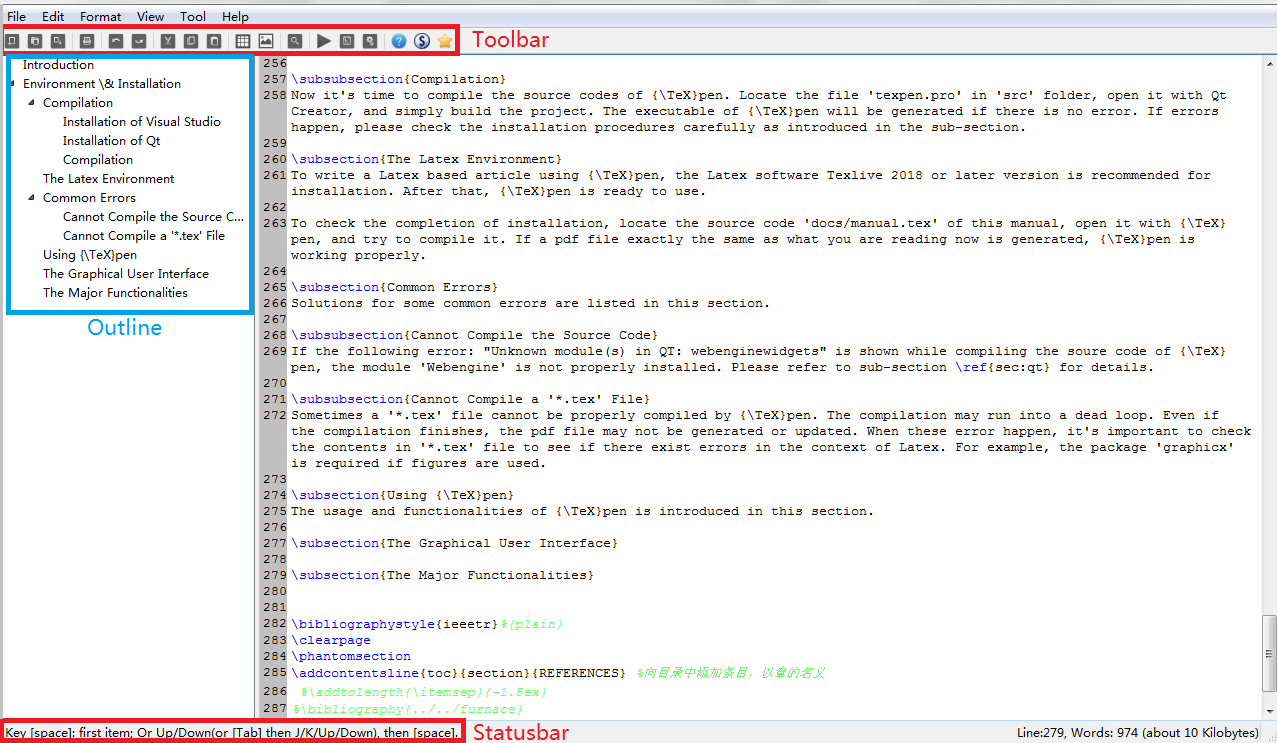
\includegraphics[scale=0.47]{figs/GUI.png}
\end{center}
\caption{The GUI of {\TeX}pen}
\label{gui}
\end{figure}


\subsection{The Major Functionalities}
All funcationalities can be accessed through the menus and shortcuts on top of the main window.

\subsubsection{File Operations}
The 'File' menu enables users to create a new '*.tex' file with an optional template, open an existing file, save the file being edited, print files, and show the list of files opened recently. There are quite a few shortcuts which help users to access files conveniently.

\subsubsection{Edit Operations}
The 'Edit' menu enables users to modify the text of the '*.tex' file with operations like undo, redo, cut, copy, paste, search etc., like what most file editers do. {\TeX}pen also offers operations specilized for Latex, for examples, inserting a table, a graphic or date/time. There are quite a few shortcuts which help users to edit files conveniently.

\subsubsection{Format}
The 'Format' menu enables users to modify the font of the text.

\subsubsection{View}
The 'View' menu enables users to adjust the appearance of the window. For examples, toolbar, outline and statusbar may be shown in the windows or hidden, according to users' needs. Color scheme of the text editing area may also be changed.

\subsubsection{Tool}
The 'View' menu probably provides the most important operations: Build, View PDF and Config. The 'Build' operation compiles the '*.tex' file being edited and generates the corresponding PDF file, which may be previewed by 'View PDF'. The 'Config' operation allows users to change the build command and working directory.

\subsubsection{Help}
The 'Help' menu allows users to view helpful tips, get details about {\TeX}pen and Qt, and make donations.


\bibliographystyle{ieeetr}%{plain}
\clearpage
\phantomsection
\addcontentsline{toc}{section}{REFERENCES} %向目录中添加条目,以章的名义
 %\addtolength{\itemsep}{-1.5ex}
%\bibliography{../../furnace}

\end{document}
 
